\chapter{Implementierung des Prototypen}

Um das im vorigen Kapitel dargestellte Konzept zu realisieren, lassen sich folgende Hauptaufgaben ausmachen. Im Folgenden wird auf Informationen oder Probleme innerhalb der einzelnen Schritte eingegangen und diese erläutern.

Es wurden viele Open Source Bibliotheken verwendet um den Fokus der Arbeit auf die Neuentwicklung und Lösung der Fragestellung zu legen.

Github wurde im Verlauf der Arbeit verwendet da das Unternehmen wie Chacon et al. in dem Buch Pro Git \cite{Chacon2014} beschreiben, der größte Dienstleister für die Bereitstellung von Git Repositories ist. Neben der Speicherung von Quellcode ist Github ebenfalls eine zentrale Plattform für den Austausch und die Zusammenarbeit von Millionen von Entwicklern. Nicht nur open-source sondern auch closed-source Projekte werden dort gespeichert und mithilfe von Problemverfolgung und Codereviews weiterentwickelt. Für die Verwaltung der Informationen verwendet Github das Versionsverwaltungstool Git und baut somit seine Funktionalität um diese Technologie herum.

\section{Einschränkungen}
Die Software kann nur funktionieren, wenn garantiert werden kann, dass keine effektiven Sicherheitsmaßnahmen verwendet werden. Folgende Maßnahmen würden das mitlesen der Kommunikation verhindern.
\begin{enumerate}
    \item Nur ohne \ac{HPKP}
    
    Auf dem Server wird ein für den Client ausgestelltes Zertifikat hinterlegt. Der öffentlichen Schlüssel oder der \glqq subjectPublicKeyInfo\grqq{}, ein weiterer Schlüssel mit Zusatzinformationen über die Verschlüsselung, dieses Zertifikats wird auf dem Client abgespeichert. Anschließend wird dieser gespeicherte Schlüssel mit jeder Anfrage an den Server mitgeschickt. Anschließend kann der Server die eingehenden Nachrichten mithilfe der Informationen aus dem Zertifikat verifizieren und sicherstellen das sie vom tatsächlichen Ziel kommt \cite{evans_palmer_sleevi_2015}.
    \item Nur wenn der Zertifizierungspfad des SSL Zertifikat (\emph{trust chain}) nicht geprüft wird.
    
    Bei Verwendung von TLS ist es möglich, den Client prüfen zu lassen, ob der Server das entsprechende Hersteller Zertifikat besitzt. Jedes gültige Zertifikat muss von einer \ac{CA} ausgestellt werden, welche das Vertrauen und eventuell die Identität des Besitzers verifiziert. Jedoch gibt es auch Implementierungen die vom Zertifikat nur die formalen Details und nicht die Herkunft (CA) prüfen.
    Dies ermöglicht, dass die Kommunikation trotz eines manuell (unverifizierbaren) Zertifikats mit den gleichen Details hergestellt werden kann.
\end{enumerate}


%%%%%%%%%%%%%%%%%%%%%%%%%%%%
%Test Client/Broker implementieren
%%%%%%%%%%%%%%%%%%%%%%%%%%%%
\section{Aufsetzen des externen Client und Broker}
    Da zum Zeitpunkt der Entwicklung keine Geräte zur Verfügung standen, wurden ein virtueller Client und Broker erzeugt, die für die Verifizierung im Labor verwendet wurden.
    Auf diese wird im Folgenden Abschnitt eingegangen.

    %Gewählte Sprache für Client und Broker
    Für die Implementierung des virtuellen Clients und externen Brokers bot sich aus folgenden Gründen Python an:
    \begin{itemize}
        \item Die Programmiersprache sollte schnell und mit geringem Aufwand zu verwenden sein.
        \item Sollte bereits über eine \ac{MQTT} Bibliothek verfügen um das Protokoll nicht selbst interpretieren zu müssen.
        \item Der Client sollte anpassbar sein.
        \item Die Sprache sollte auf Linux laufen um ein Ressourcen sparende Verwendung zu ermöglichen.
        \item Sie sollte ebenfalls auf verschiedenen Betriebssystemen lauffähig \emph{cross platform} sein, um auf beliebigen Systemen verwendbar zu sein.
    \end{itemize}
    %https://pdfs.semanticscholar.org/409d/3f740518eafcfaadb054d9239009f3f34600.pdf
    Nach Sanner ist Python ist eine interaktive und objektorientierte Programmiersprache. Sie wird anders als übliche Programmiersprachen somit nicht zuvor kompiliert\footnote{In maschinenlesbare Instruktionen umwandeln.} sondern zur Laufzeit interpretiert.
    Es stehen verschiedene Datenstrukturen aus high-level Programmiersprachen zur Verfügung wie z.B.: dynamische Bindungen, automatisches Memory Management, Klassen, Ausnahmebehandlung. Weiter ist sie eine einfache, leistungsstarke und universelle Programmiersprache, die einen elegante Syntax vorweist. \cite{sanner1999python}
        
    %Open-Source Bibliotheken Client/Broker
    Eclipse Paho ist eine quelloffene Implementierung eines Clients nach dem \ac{MQTT}-Standard. Dieser Client ist in verschiedenen Programmiersprachen verfügbar und bringt abhängig von dieser, ausgewählte Funktionalitäten mit.
    Das Protokol \ac{MQTT} in der Version 5 wird aktuell bereits in der Sprache C, jedoch von keiner anderen Implementierung unterstützt. Python unterstützt Version 3 des Standards und alle weiteren Features abgesehen von \glqq Message persistance\grqq{} und \glqq high availability\grqq{} was jedoch zu Testzwecken nicht benötigt wird. \cite{eclipse_foundation2017}
    Diese Bibliothek vereinfacht das Programmieren der Clients ungemein mithilfe der vordefinierten Klassen und Funktionen.
    Aus diesem Grund kann sehr viel Konfiguriert und somit auf den eigenen Bedarf eingestellt werden. 

    HBMQTT ist ebenfalls eine Implementierung des \ac{MQTT} Standards, allerdings stellt diese Bibliothek auch einen Broker zur Verfügung. Der Vor- und gleichzeitiger Nachteil ist, dass in dieses Framework sehr restriktiv und eingeschränkt Konfigurierbar ist. Dadurch ist es einfach ein Broker aufzusetzen, jedoch nicht ohne weiteres anzupassen.
    \cite{jouanin_2018}
    
%%%%%%%%%%%%%%%%%%%%%%%%%%%%
%Implementieren des Proxys (Backend)
%%%%%%%%%%%%%%%%%%%%%%%%%%%%
\section{Implementierung des Backends}

    Es wurden verschiedene Programmiersprachen für den Proxy verwendet. Diese wurde entsprechend der Anforderungen und dem Einsatzgebiet abhängig gewählt.
    Die wichtigste Unterscheidung liegt an der Trennung von Backend (Server und Logik Komponenten) und Frontend (Webseite oder User Interface).
    Zuerst wird auf die Sprache für das Backend eingegangen.
    
%%%%%%%%%%%
%Visual Studio
%%%%%%%%%%%
    Als Entwicklungsumgebung für das Backend wurde Visual Studio 2017 \cite{microsoft_2019} von Microsoft verwendet. Dadurch sind auch die Projektdateien, die in dem Repository \glqq MQTT-Proxy\grqq{} \cite{eisenschmidt_2019} gefunden werden können, in einem Visual Studio Projektfile (.sln) definiert.
    
%%%%%%%%%%%
%Anforderungen an die Programmiersprache
%%%%%%%%%%%
    \begin{itemize}
        \item Die Sprache muss verschiedene Bibliotheken mitbringen die Funktionalitäten wie REST-Interface und \ac{MQTT}-Protokoll bereitstellen. Dies ist aufgrund der kurzen Zeit die für diese Arbeit veranschlagt wurde notwendig um alle Features implementiert zu bekommen.
        \item Das Programm muss auf mindestens zwei Plattformen verwendbar sein um den praktischen Nutzen zu steigern.
        \item Es soll eine bekannte Sprache sein, um eine Weiterentwicklung von Dritten zu ermöglichen.
        \item Die Programmiersprache muss dem Autor bereits bekannt sein, um die Einarbeitungszeit minimal zu halten und auch eine entsprechende Qualität zur Verfügung stellen zu können.
    \end{itemize}
%%%%%%%%%%%
%Sprache
%%%%%%%%%%%
    %Welche Sprachen wären basierend darauf möglich/naheliegend gewesen
    Basieren auf diesen Anforderungen stehen Java, C\# und JavaScript zur Auswahl.
    Der Autor hat sich anschließend aus folgenden Gründen für C\# entschieden.
    %Warum sind die Entwickelt worden? / Vorteile Background
    %Was macht die Programmiersprachen aus? / Schwerpunkt
    \begin{itemize}
        \item Die \ac{IDE} Visual Studio und das .NET Framework sind stark in Windows integriert, wodurch die Verwendung dieser unter Windows erleichtert wird.
        \item Das .NET Framework besitzt ein Assembly System bei dem Bibliotheken in einzelne Dateien ausgelagert und dynamisch geladen werden können.
        \item Es ist kein Linking nötigt, da externe Abhängigkeiten zur Laufzeit aufgelöst werden.
        \item Das Paketmanagement System Nuget ermöglicht eine schnelle und einfache Verwaltung sowie Einbindung externer Bibliotheken.
    \end{itemize}
    
    
%%%%%%%%%%%
%Nuget %https://link.springer.com/book/10.1007%2F978-1-4302-4192-8
%%%%%%%%%%%
    NuGet wurde aus den folgenden Vorteilen ausgewählt, welche ebenfalls von Balliauw et al. beschrieben werden \cite{balliauw2012pro}.
    Der sogenannte Paket-Manager unterstützt bei der Verwaltung von Abhängigkeiten, wie zum Beispiel Bibliotheken, mit dem Auflösen von Abhängigkeiten und Versionsproblemen. Versionsprobleme treten dann auf, wenn Bibliotheken Abhängigkeiten mit einer Version < X und eine weitere Bibliothek Version > X benötigen. Ein weitere oft auftretender Fall ist, dass beim Aktualisieren einer Bibliothek die benötigte Version für die Abhängigkeiten erhöht aber nicht ebenfalls aktualisiert wird. Die Folge ist eine defekte Abhängigkeit für die Bibliothek und also ein nicht kompilierbarer Zustand  und somit nicht ausführbares Programm. Zusätzlich übernimmt es auch die Installation durch Suchen, Installieren und Aktualisieren oder Entfernen von gewünschten Paketen. Ein weiterer Vorteil ist, dass der Quellcode öffentlich verfügbar ist und das Tool somit weiter angepasst oder verändert werden kann.
    
%%%%%%%%%%%
%Bibliothek
%%%%%%%%%%%
    NewsoftJSON \cite{newton_king_2013} ist ein quelloffenes Framework für die Serialisierung und Deserialisierung von .NET Framework Objekten.
    Heinzl beschreibt Serialisierung mit folgenden Worten \glqq Unter Serialisierung versteht man die Zerlegung des Status eines Objekts in ein Bytearray.\grqq{} \cite{Heinzl2005}. Allerdings ist es auch möglich dieses Bytearray als strukturierten Text anzeigen zu lassen.
    Dies ermöglicht, ein Nachrichtenobjekt an das Frontend zu übertragen und es dort anschließend wieder darstellen zu lassen.
    
    MQTTNet ist eine quelloffene Implementierung des \ac{MQTT}-Standards in C\# unter der MIT Lizenz\footnote{
    Github beschreibt die Lizenz als einfache freigebige Lizenz mit nur wenigen Einschränkungen wie dem Erhalt von Urheberrechts- und Lizenzhinweisen. Änderungen und größere Werke können unter anderen Lizenzbedingungen und ohne Quellcode verbreitet werden. \cite{github_inc_2019}}.
    Da die Bibliothek MQTTnet \cite{chkr1011_2018},
    welche in dieser Arbeit verwendet wird, die Bridge Funktionalität nicht besitzt ist es notwendig sie selbst zu implementieren. Um das gleiche Ergebnis wie die der Bridge zu erreichen muss an den Broker eine Client Komponente angeschlossen werden der die Kommunikation nach außen steuert und die Antworten weiter verarbeitet. 
    
    WebSocketSharp ist eine C\# Implementierung des WebSocket Protokolls und unterstützt sowohl den Client als auch die Bereitstellung des Server.
    
    Grapevine ist eine .NET Bibliothek die zwei Probleme verfolgt.
    \begin{itemize}
        \item Das einfache einbinden eines REST und HTTP Servers.
        \item Die einfache Verwendung von REST Ressourcen.
    \end{itemize}
    Der Fokus liegt dabei auf der Bereitstellung von Ressourcen über HTTP oder REST für Programme, die einen anderen Schwerpunkt haben und dies nur als Zusatzfunktion benötigen.
    
%%%%%%%%%%%%%%%%%%%%%%%%%%%%
%Implementieren des Proxys (Frontend)
%%%%%%%%%%%%%%%%%%%%%%%%%%%%
\section{Implementierung des Frontends}
    
    Nun wird auf die Programmiersprache für das Frontend, also die Oberfläche eingegangen.
    
%%%%%%%%%%%
%Visual Studio Code
%%%%%%%%%%%
    %https://proquestcombo.safaribooksonline.com/9781484242247
    Zum Entwickeln des Frontends, also der Weboberfläche mit der Nutzer interagieren und die Applikation steuern können, wurde Visual Studio Code \cite{microsoft_2016} verwendet.
    
%%%%%%%%%%%
%Anforderungen an die Programmiersprache
%%%%%%%%%%%
    \begin{itemize}
        \item Es muss möglich sein, einzelne Inhalte auf der Webseite dynamisch, also ohne Aktualisierung der Webseite, austauschen zu können.
        \item Wenn neu abgefangenen Nachrichten im Proxy verfügbar sind, sollen sie automatisch an das Frontend weitergegeben werden und das Datenmodel der Oberfläche automatisch aktualisieren.
        \item Die Oberfläche soll aus Komponenten bestehen und mithilfe dieser einen modularen und strukturierten Aufbau ermöglichen.
        \item Funktionalitäten und Ausprägungen von Komponenten sollen gekapselt sein.
    \end{itemize}
    
%%%%%%%%%%%
%Welche Sprachen wären basierend darauf möglich/naheliegend gewesen
%%%%%%%%%%%
    Durch die existierenden Anforderungen hat sich JavaScript als passend herausgestellt. Dadurch, dass verschiedene Frameworks und Erweiterungen auf Basis von JavaScript existieren, werden im Folgenden noch die konkreten Frameworks auf die Anforderungen untersucht.
    
%%%%%%%%%%%
%Warum Vue.js
%%%%%%%%%%%
    Vue.js \cite{you2018vue} wurde ursprünglich für schnelles Prototyping von Webseiten entwickelt, hat sich aber mit der Zeit in die Liste der beliebtesten Webtechnologien eingereiht. Neben Angular und React, stellt es eine Alternative zum schnellen und leichtgewichtigen Entwickeln mit \ac{MVVM}-Architekturmuster dar. Dies ermöglicht die Wiederverwendung von Code durch Nutzung von Komponenten. Durch die bidirektionale Databindung ist es möglich Änderungen im Clientmodel direkt, ohne Aktualisierung, anzeigen zu lassen. In der gegengesetzten Richtung, werden die Informationen, welche zum Beispiel in Inputfeldern bearbeitet werden können, direkt im Clientmodel abgespeichert. Ein weiterer Vorteil ist die direkte Abbildung vom Datenmodel also Datenstruktur zum ViewModel. Dies ermöglicht auch eine Trennung von UI-Designern und Entwicklern da getrennt entwickelt werden kann ohne Informationen in Bereichen der anderen abändern zu müssen.
    %%%%%%%%%%%%%%%%%%%%%%%%%%%%%%%%%%%%%%%
    % Danke an Moritz für die Infos \.A./ %
    %%%%%%%%%%%%%%%%%%%%%%%%%%%%%%%%%%%%%%%
    
%%%%%%%%%%%
%Bibliothek
%%%%%%%%%%%
    Als Bibliothek wurde Bootstrap-Vue gewählt, um schnell anpassbare Oberflächen erstelle zu können.
    Laut Morehouse \cite{morehouse_2019} ist sie die umfassendste Implementierung von Bootstrap in der Version 4 für Vue.js.
    Bootstrap ist ein quelloffenes Framework, welches fertige Vorlagen und Komponenten für die Erstellung von Webseiten bereitstellt. Der Unterschied zwischen Bootstrap und Bootstrap-Vue besteht darin, dass die vorhandenen Elemente nun als Komponenten in Vue vorhanden sind und somit nicht der ursprüngliche \ac{HTML}-Code\footnote{\ac{HTML} ist die Auszeichnungssprache für das \ac{WWW} \cite{w3c_2017}. Was bedeutet, dass es die grundlegende Sprache für das Erstellen von Webseiten ist.} geschrieben werden muss. Diese Informationen werden automatisch mithilfe der Vue Komponenten generiert.
        
%%%%%%%%%%%%%%%%%%%%%%%%%%%%
%Kommunikation mit Firewall
%%%%%%%%%%%%%%%%%%%%%%%%%%%%
\section{Umsetzung des MITM Proxies}
    %MITM (APR Spoof, DNS, ICMP, FW)
    Es gibt verschiedene Techniken und Möglichkeiten, die Kommunikation so zu verändern, dass ein drittes Gerät die übertragenen Nachrichten mitlesen kann. Ein solches Konzept ist auch unter dem Namen \emph{Man in the Middle} bekannt.
    
    Eine der Möglichkeiten wird auch in dieser Arbeit umgesetzt das die Verbindung vom Client direkt zum Broker aufgebaut wird.
    Mithilfe von Portweiterleitungung in der Firewall \emph{OPNSense} wurden Netzwerkpakete des \ac{IoT}-Gerätes an den Proxy umgeleitet. Hierzu wurde eine Regel erzeugt (siehe \ref{fig:firewall_rule}, die das \emph{source} Attribut jedes eintreffenden Pakets mit der IP-Addresse des Geräts und dem Standard-Port 1883 vergleicht. Bei Übereinstimmung wurde das \emph{destination} Attribut der Pakete umgeschrieben um die Pakete anschließend an den Proxy weiterzuleiten.
    \begin{figure}[h]%h=direkt danach t=top b=bottom
        \centering
        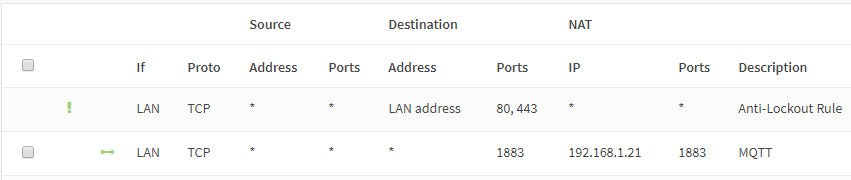
\includegraphics[width=14cm]{tex/bilder/5_implementierung/firewall.PNG}
        \captionof{figure}{Firewallregel zum Umleiten der MQTT-Pakete}
        \label{fig:firewall_rule}
    \end{figure}